% MNRAS manuscript, version 2 (step-by-step).  Build:  tectonic mnras_a0_lambda_v2.tex
% (or pdflatex + bibtex + pdflatex x2 with mnras.cls installed).  Numbers: paper_numbers.py; figures: make_figures.py.
\documentclass[fleqn,usenatbib]{mnras}
\usepackage{newtxtext,newtxmath}
\usepackage[T1]{fontenc}
\usepackage{graphicx}
\usepackage{booktabs}
\usepackage{amsmath}
\usepackage{hyperref}

% The corresponding author's e-mail is kept out of the public repository.  make_upload_bundle.py substitutes it into a
% copy of this file inside the git-ignored upload_bundle/ and builds the submission PDF there.
\newcommand{\authoremail}{address supplied at submission}

\title[The $a_0$--$\Lambda$ relation and its redshift test]{The galactic acceleration scale and the cosmological constant: the coefficient measured, its degeneracy with $H_0$, and a redshift test}

\author[C. P. Zimmerman]{Carl P. Zimmerman$^{1}$\thanks{E-mail: \authoremail}
\\
$^{1}$Briar Creek Tech, USA}

\date{Accepted XXX. Received YYY; in original form ZZZ}
\pubyear{2026}

\begin{document}
\label{firstpage}
\pagerange{\pageref{firstpage}--\pageref{lastpage}}
\maketitle

\begin{abstract}
The acceleration scale $a_0$ of the radial acceleration relation is numerically close to $c\sqrt{G\rho_\Lambda}$, the only acceleration built from $c$, $G$ and the density of the cosmological constant. We write $a_0=\kappa c\sqrt{G\rho_\Lambda}$ and ask three empirical questions. (i) What is $\kappa$? On the SPARC galaxies the Tully--Fisher intercept gives $\kappa=0.47\pm0.08$; a shape-only estimator, immune to the distance scale but fragile to the bulge mass-to-light ratio, gives $0.55\pm0.17$. The value $\kappa=1/2$ ($a_0=9.36\times10^{-11}$ m s$^{-2}$) is consistent with both. In the deep regime of SPARC and MIGHTEE-HI the slope matches the prediction, and at comparable stellar mass-to-light ratios the amplitude gives $\kappa\simeq0.5$--$0.6$. The stellar and gas mass calibrations set a 9.5 per cent floor on $a_0$ that no sample size removes. (ii) At fixed $\Omega_\Lambda$ the prediction depends only on $\kappa H_0$, so $\kappa$ cannot be quoted without $H_0$: $\kappa=1/2$ with the Planck $H_0$ and $0.461$ with the SH0ES $H_0$ give the same $a_0$. (iii) A $\Lambda$-anchored scale does not evolve, whereas a scale tied to the critical density grows as $H(z)$ ($+0.58$ dex at $z=2.5$) and the emergent scale of $\Lambda$CDM haloes grows by $+0.33$ dex. We derive the error amplification that stops existing high-redshift samples from deciding, show that the verdict of the largest (99 rotation curves at $0.6<z<2.5$) is erased by a 0.05 dex per unit redshift drift in the baryonic-mass calibration, and specify the deciding measurement: two to four lensed rotators at $z\simeq2.5$ with baryonic accelerations below $0.3a_0$, each measured to $0.10$--$0.20$ dex. The coefficient is not derived.
\end{abstract}

\begin{keywords}
gravitation -- galaxies: kinematics and dynamics -- galaxies: high-redshift -- cosmological parameters -- dark energy -- dark matter
\end{keywords}

%=====================================================================================================================
\section{Introduction}
\label{sec:intro}
In rotationally supported galaxies the observed centripetal acceleration, $g_{\rm obs}=V^2/R$, is a function of the acceleration $g_{\rm bar}$ that the visible stars and gas would produce on their own. This radial acceleration relation \citep{McGaugh2016,Lelli2017} contains one dimensional constant, $a_0\simeq1.2\times10^{-10}$ m s$^{-2}$. Above $a_0$ the two accelerations agree; far below it, $g_{\rm obs}\simeq\sqrt{g_{\rm bar}a_0}$, which is also the content of the baryonic Tully--Fisher relation \citep{McGaugh2012,Lelli2019}. The same constant was introduced by \citet{Milgrom1983} as the scale of a modified dynamics (MOND), and he noted at once that $a_0$ is of the order of $cH_0$. In their review, \citet{FamaeyMcGaugh2012} describe $a_0$ as of the order of the square root of the cosmological constant in natural units, and \citet{Milgrom2020} writes the coincidence in two forms, $2\pi a_0\simeq cH_0$ and $2\pi a_0\simeq c^2\sqrt{\Lambda/3}$.

Those two forms are different physical statements. If $a_0$ follows the expansion rate it was larger in the past, by a factor $3.8$ at $z=2.5$. If it follows the cosmological constant it never changes. Today the two differ only by the factor $\Omega_\Lambda^{-1/2}=1.21$, which is inside the uncertainty of any measurement of $a_0$, so local data cannot tell them apart. A third possibility is that there is no fundamental $a_0$ at all: in $\Lambda$CDM the relation is an emergent property of galaxies in dark-matter haloes \citep{Navarro2017,Ludlow2017,KellerWadsley2017}, and the characteristic acceleration of haloes also grows with redshift.

This paper takes the $\Lambda$ reading as a hypothesis and asks what can be measured. We write
\begin{equation}
a_0=\kappa\,c\sqrt{G\rho_\Lambda},
\label{eq:relation}
\end{equation}
where $\rho_\Lambda$ is the mass density equivalent to the cosmological constant and $\kappa$ is a pure number, and we address three questions.
\begin{enumerate}
\item \emph{What is $\kappa$, and how well can it be known?} (Section~\ref{sec:kappa}.)
\item \emph{How does the answer depend on the Hubble constant?} (Section~\ref{sec:h0}.)
\item \emph{Which observation separates equation~(\ref{eq:relation}) from the alternatives?} (Section~\ref{sec:ztest}.)
\end{enumerate}
Section~\ref{sec:relation} sets out the relation and its equivalent forms, Section~\ref{sec:limits} lists what it does not explain, and Section~\ref{sec:conc} concludes.

The idea has a long history and we claim no priority for it. \citet{Milgrom1999} obtained MOND-like behaviour from the Unruh temperature of an accelerated observer in de Sitter space, with a coefficient corresponding to $a_0=2cH_\Lambda$. \citet{Limbach2008} proposed the redshift evolution of the Tully--Fisher relation as a test of whether $a_0$ is coupled to the dark-energy density or to the Hubble rate. \citet{BlanchetLeTiec2009}, \citet{KlinkhamerKopp2011}, \citet{Verlinde2017} and \citet{Milgrom2020} relate $a_0$ to $\Lambda$ or to $H_0$ with coefficients of their own. \citet{OppenheimRusso2024} argued that stochastic fluctuations of spacetime in a classical--quantum theory of gravity produce a term acting as a cosmological constant together with one of the kind used to fit rotation curves without dark matter; \citet{HertzbergLoeb2024} dispute both the derivation and that the term has the MOND form. What this paper adds is a measurement of the coefficient with a complete error budget, the statement of its degeneracy with $H_0$, and a quantitative design for the redshift test, including the reasons existing samples cannot perform it. We do not derive $\kappa$, and we take no position on whether the low-acceleration behaviour of galaxies reflects modified gravity, modified inertia or the physics of dark matter.

Every number below is produced by a public script with checks that can fail (Appendix~\ref{app:repro}). We carry both densities throughout: $\rho_\Lambda$, and the critical density $\rho_{\rm crit}$ as the named alternative.

%=====================================================================================================================
\section{The relation, step by step}
\label{sec:relation}
\subsection{The density of the cosmological constant}
The Friedmann equation for a spatially flat universe is $H^2=8\pi G\rho/3$. The total density today is therefore the critical density,
\begin{equation}
\rho_{\rm crit}=\frac{3H_0^2}{8\pi G},
\label{eq:rhocrit}
\end{equation}
and the part of it in the cosmological constant is
\begin{equation}
\rho_\Lambda=\Omega_\Lambda\,\rho_{\rm crit}=\frac{\Lambda c^2}{8\pi G}.
\label{eq:rholambda}
\end{equation}
Unlike the matter density, $\rho_\Lambda$ does not dilute as the Universe expands. We define the associated expansion rate $H_\Lambda$ by $H_\Lambda^2=8\pi G\rho_\Lambda/3$, so that
\begin{equation}
H_\Lambda=H_0\sqrt{\Omega_\Lambda}=c\sqrt{\Lambda/3}.
\label{eq:hlambda}
\end{equation}
This is the constant rate that the expansion approaches in the far future.

\subsection{The only acceleration available}
Which accelerations can be formed from $c$, $G$ and a density $\rho$? Write $a=c^{\alpha}G^{\beta}\rho^{\gamma}$. The dimensions are $[c]={\rm m\,s^{-1}}$, $[G]={\rm m^{3}\,kg^{-1}\,s^{-2}}$, $[\rho]={\rm kg\,m^{-3}}$ and $[a]={\rm m\,s^{-2}}$. Matching the powers of each unit gives three equations,
\begin{align}
\text{kilograms:}\quad & -\beta+\gamma=0,\\
\text{seconds:}\quad & -\alpha-2\beta=-2,\\
\text{metres:}\quad & \alpha+3\beta-3\gamma=1.
\end{align}
The first gives $\gamma=\beta$. The third then gives $\alpha=1$, and the second gives $\beta=1/2$. The solution is unique: every acceleration built from these three quantities has the form $\kappa c\sqrt{G\rho}$ with $\kappa$ a pure number. Dimensional analysis fixes the form of equation~(\ref{eq:relation}) and says nothing about $\kappa$. The physical content of the hypothesis lies in two places: the value of $\kappa$, and the choice of $\rho_\Lambda$ rather than another density.

\subsection{Four ways of writing the same thing}
\label{sec:forms}
Equation~(\ref{eq:relation}) can be rewritten with equations~(\ref{eq:rholambda}) and (\ref{eq:hlambda}). Each line below is algebra and carries no new information.

\emph{In terms of $\Lambda$.} From equation~(\ref{eq:rholambda}), $G\rho_\Lambda=\Lambda c^2/8\pi$, so
\begin{equation}
a_0=\kappa\,c^2\sqrt{\frac{\Lambda}{8\pi}}\qquad\Big(\kappa=\tfrac12:\ a_0=c^2\sqrt{\Lambda/32\pi}\Big).
\end{equation}

\emph{In terms of $H_\Lambda$.} From $H_\Lambda^2=8\pi G\rho_\Lambda/3$ we have $\sqrt{G\rho_\Lambda}=H_\Lambda\sqrt{3/8\pi}$, so
\begin{equation}
a_0=\frac{cH_\Lambda}{Z},\qquad Z\equiv\frac{1}{\kappa}\sqrt{\frac{8\pi}{3}}\qquad\Big(\kappa=\tfrac12:\ Z=\sqrt{32\pi/3}=5.79\Big).
\label{eq:Z}
\end{equation}

\emph{In terms of the de Sitter radius} $R_{\rm dS}=c/H_\Lambda$:
\begin{equation}
a_0=\frac{c^2}{Z\,R_{\rm dS}} .
\end{equation}

\emph{In natural units} ($\hbar=c=1$), with $\rho_\Lambda=M_\Lambda^4$ and $G=M_{\rm P}^{-2}$:
\begin{equation}
a_0=\kappa\,\frac{M_\Lambda^2}{M_{\rm P}} .
\end{equation}
A warning belongs here. Because $Z$ is defined from $\kappa$ by equation~(\ref{eq:Z}), the statement `$cH_\Lambda/a_0=5.79$' is the statement `$\kappa=1/2$' in other units. Agreement between these forms confirms nothing; only a measurement of $a_0$ does.

\subsection{The numbers}
\label{sec:numbers}
Table~\ref{tab:inputs} evaluates equation~(\ref{eq:relation}) one step at a time from the \citet{Planck2020} parameters, rounded to $H_0=67.4$ km s$^{-1}$ Mpc$^{-1}$ and $\Omega_\Lambda=0.685$. For $\kappa=1/2$,
\begin{equation}
a_0=\tfrac12c\sqrt{G\rho_\Lambda}=9.36\times10^{-11}\ {\rm m\,s^{-2}} .
\label{eq:a0value}
\end{equation}
The alternative built on the critical density is larger by $\Omega_\Lambda^{-1/2}=1.208$:
\begin{equation}
\tfrac12c\sqrt{G\rho_{\rm crit}}=\frac{cH_0}{5.79}=1.13\times10^{-10}\ {\rm m\,s^{-2}} .
\label{eq:a0crit}
\end{equation}
Both lie within about one systematic standard deviation of the standard determination, $a_0=(1.20\pm0.02\pm0.24)\times10^{-10}$ m s$^{-2}$ \citep{McGaugh2016}. The 21 per cent between them is the quantity that local data cannot resolve (Section~\ref{sec:kappa}) and that the redshift test of Section~\ref{sec:ztest} magnifies to a factor of 3.8.

\begin{table}
\caption{Equation~(\ref{eq:relation}) evaluated step by step. Inputs: $c=2.99792458\times10^{8}$ m s$^{-1}$, $G=6.6743\times10^{-11}$ m$^3$ kg$^{-1}$ s$^{-2}$, 1 Mpc $=3.08568\times10^{22}$ m, $H_0=67.4$ km s$^{-1}$ Mpc$^{-1}$, $\Omega_\Lambda=0.685$.}
\label{tab:inputs}
\begin{tabular}{lll}
\toprule
step & quantity & value\\
\midrule
1 & $H_0=67.4\times10^{3}/3.08568\times10^{22}$ & $2.184\times10^{-18}$ s$^{-1}$\\
2 & $\rho_{\rm crit}=3H_0^2/8\pi G$ & $8.533\times10^{-27}$ kg m$^{-3}$\\
3 & $\rho_\Lambda=\Omega_\Lambda\rho_{\rm crit}$ & $5.845\times10^{-27}$ kg m$^{-3}$\\
4 & $G\rho_\Lambda$ & $3.901\times10^{-37}$ s$^{-2}$\\
5 & $\sqrt{G\rho_\Lambda}$ & $6.246\times10^{-19}$ s$^{-1}$\\
6 & $c\sqrt{G\rho_\Lambda}$ & $1.872\times10^{-10}$ m s$^{-2}$\\
7 & $a_0=\tfrac12c\sqrt{G\rho_\Lambda}$ & $9.36\times10^{-11}$ m s$^{-2}$\\
\midrule
  & $cH_0$ & $6.55\times10^{-10}$ m s$^{-2}$\\
  & $cH_\Lambda=cH_0\sqrt{\Omega_\Lambda}$ & $5.42\times10^{-10}$ m s$^{-2}$\\
  & $\Lambda=3H_\Lambda^2/c^2$ & $1.09\times10^{-52}$ m$^{-2}$\\
  & $R_{\rm dS}=c/H_\Lambda$ & $1.66\times10^{26}$ m $=5.37$ Gpc\\
  & $M_\Lambda=\rho_\Lambda^{1/4}$ & $2.24$ meV\\
\bottomrule
\end{tabular}
\end{table}

\subsection{The classical coincidences as values of $\kappa$}
\label{sec:cands}
Earlier statements of the coincidence translate into values of $\kappa$ through equation~(\ref{eq:Z}): an acceleration $a_0=cH_\Lambda/Z$ has $\kappa=\sqrt{8\pi/3}/Z$, and $cH_0=cH_\Lambda/\sqrt{\Omega_\Lambda}$. Thus the two forms of \citet{Milgrom2020}, $a_0=cH_\Lambda/2\pi$ and $a_0=cH_0/2\pi$, correspond to $\kappa=\sqrt{8\pi/3}/2\pi=0.461$ and to $\kappa=0.557$; the acceleration whose Unruh temperature equals the temperature of the de Sitter horizon, $a_0=cH_\Lambda$, to $\kappa=2.89$; the $cH_0/6$ of \citet{Verlinde2017} to $\kappa=0.583$; and the $2cH_\Lambda$ of \citet{Milgrom1999} to $\kappa=5.79$, a factor 12 too large. These are collected with the measurements in Table~\ref{tab:cands}.

%=====================================================================================================================
\section{Measuring the coefficient}
\label{sec:kappa}
\subsection{Data and fitting function}
We use the SPARC database \citep{Lelli2016}: 175 disc galaxies with 3.6 $\mu$m photometry and H\,{\sc i}/H$\alpha$ rotation curves. At each radius $R$ the database gives the observed velocity $V_{\rm obs}$ and the Newtonian velocities $V_{\rm gas}$, $V_{\rm disc}$, $V_{\rm bul}$ of the gas and of the stellar components for unit stellar mass-to-light ratio. The two accelerations are
\begin{equation}
g_{\rm obs}=\frac{V_{\rm obs}^2}{R},\qquad
g_{\rm bar}=\frac{V_{\rm gas}|V_{\rm gas}|+\Upsilon_{\rm disc}V_{\rm disc}^2+\Upsilon_{\rm bul}V_{\rm bul}^2}{R},
\label{eq:gdef}
\end{equation}
where $\Upsilon_{\rm disc}$ and $\Upsilon_{\rm bul}$ are the stellar mass-to-light ratios at 3.6 $\mu$m in solar units. Keeping points with a velocity error below 10 per cent leaves 2803 points in 164 galaxies, spanning $8\times10^{-13}<g_{\rm bar}<7\times10^{-9}$ m s$^{-2}$ (Fig.~\ref{fig:rar}).

We describe the relation with the function used by \citet{McGaugh2016}, whose form is due to \citet{MilgromSanders2008}:
\begin{equation}
g_{\rm obs}=\nu(y)\,g_{\rm bar},\qquad \nu(y)=\frac{1}{1-e^{-\sqrt y}},\qquad y\equiv\frac{g_{\rm bar}}{a_0}.
\label{eq:nu}
\end{equation}
Its two limits are worth writing out. For $y\gg1$ the exponential vanishes, $\nu\to1$ and $g_{\rm obs}=g_{\rm bar}$. For $y\ll1$, put $s=\sqrt y$ and expand $1-e^{-s}=s-s^2/2+\ldots$; then
\begin{equation}
\nu=\frac{1}{s}\Big(1+\frac{s}{2}+\ldots\Big)\quad\Longrightarrow\quad g_{\rm obs}=\sqrt{g_{\rm bar}a_0}\,\Big(1+\tfrac12\sqrt y+\ldots\Big).
\label{eq:deep}
\end{equation}
The leading term is the deep regime, in which $a_0=g_{\rm obs}^2/g_{\rm bar}$. The correction falls only as $\sqrt y$: at $y=0.01$ it is still 5 per cent in $g_{\rm obs}$ and 10 per cent in $a_0$. This slow approach matters repeatedly below. We use equation~(\ref{eq:nu}) as an empirical description of galaxy data and nothing more; Section~\ref{sec:limits} returns to this.

\begin{figure}
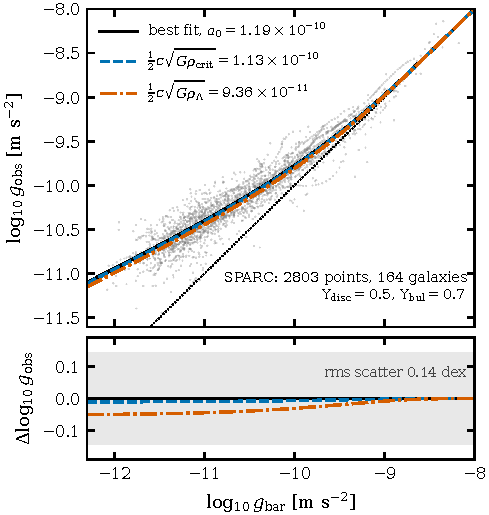
\includegraphics[width=\columnwidth]{fig1_rar.pdf}
\caption{The radial acceleration relation of SPARC (grey points; $\Upsilon_{\rm disc}=0.5$, $\Upsilon_{\rm bul}=0.7$) with equation~(\ref{eq:nu}) for three values of $a_0$: the best fit at this mass-to-light ratio (solid), $\tfrac12c\sqrt{G\rho_{\rm crit}}$ (dashed) and $\tfrac12c\sqrt{G\rho_\Lambda}$ (dot-dashed). The dotted line is $g_{\rm obs}=g_{\rm bar}$. Lower panel: the curves relative to the best fit; the band is the rms scatter of the data. The curves differ by at most 0.05 dex, a third of the scatter.}
\label{fig:rar}
\end{figure}

\subsection{The standard fit and its degeneracy with the mass-to-light ratio}
\label{sec:standard}
The simplest estimate minimises the residuals in $\log_{10}g_{\rm obs}$ over $a_0$ at fixed mass-to-light ratios. With $\Upsilon_{\rm disc}=0.5$ and $\Upsilon_{\rm bul}=0.7$ we recover the value of \citet{McGaugh2016}, $a_0=1.19\times10^{-10}$ m s$^{-2}$ with an rms scatter of 0.14 dex. The result depends steeply on $\Upsilon_{\rm disc}$ (Table~\ref{tab:upsilon}, Fig.~\ref{fig:kappa}a), and equation~(\ref{eq:deep}) shows why. Where stars dominate, $g_{\rm bar}\propto\Upsilon$; in the deep regime the data fix the product $g_{\rm bar}a_0=g_{\rm obs}^2$; so $a_0\propto1/\Upsilon$.

\begin{table}
\caption{The standard fit of equation~(\ref{eq:nu}) to SPARC as a function of the disc mass-to-light ratio ($\Upsilon_{\rm bul}=0.7$). $\kappa_\Lambda$ and $\kappa_{\rm crit}$ are $a_0$ divided by $c\sqrt{G\rho_\Lambda}$ and by $c\sqrt{G\rho_{\rm crit}}$.}
\label{tab:upsilon}
\begin{tabular}{ccccc}
\toprule
$\Upsilon_{\rm disc}$ & $a_0$ [$10^{-10}$ m s$^{-2}$] & $\kappa_\Lambda$ & $\kappa_{\rm crit}$ & rms [dex]\\
\midrule
0.40 & 1.49 & 0.795 & 0.658 & 0.148\\
0.50 & 1.19 & 0.636 & 0.526 & 0.144\\
0.60 & 0.97 & 0.520 & 0.431 & 0.143\\
0.70 & 0.81 & 0.434 & 0.359 & 0.145\\
0.80 & 0.69 & 0.367 & 0.304 & 0.148\\
\bottomrule
\end{tabular}
\end{table}

The quality of the fit is almost flat across the table, so the data do not choose $\Upsilon_{\rm disc}$. Stellar population models give $\Upsilon_{\rm disc}\simeq0.5$--$0.7$ at 3.6 $\mu$m \citep{Meidt2014,Schombert2019}. In this estimator $\kappa=1/2$ requires $\Upsilon_{\rm disc}=0.62$ for the $\rho_\Lambda$ reading and $0.52$ for the $\rho_{\rm crit}$ reading. Both are inside the allowed range, and that is all the standard fit can say. Restricting the fit to the deep band, $g_{\rm bar}<0.1a_0$, where the stars carry less of the mass, does not remove the dependence: $\kappa=0.56$, $0.49$ and $0.44$ for $\Upsilon_{\rm disc}=0.5$, $0.6$ and $0.7$. (Giving the points whose velocity errors exceed 10 per cent equal weight lowers each value by about 0.1.) Two estimators that depend on the mass-to-light ratio in different ways do better.

\subsection{Estimator A: the Tully--Fisher intercept, with its finite-depth correction}
\label{sec:btfr}
The baryonic Tully--Fisher relation is often quoted as $V_f^4=GM_ba_0$ for the flat rotation velocity $V_f$ and the baryonic mass $M_b$. That is a limit. The exact statement follows from equation~(\ref{eq:nu}) in three steps, evaluated at the outermost measured radius $R$.

\emph{Step 1.} $g_{\rm obs}=V_f^2/R$ and $g_{\rm obs}=\nu(y)g_{\rm bar}$ give $V_f^4=\nu^2g_{\rm bar}^2R^2$.

\emph{Step 2.} Split $g_{\rm bar}^2R^2=g_{\rm bar}\times(g_{\rm bar}R^2)$. The first factor is $y\,a_0$. For the second, define the geometry factor $\Gamma\equiv g_{\rm bar}R^2/(GM_b)$. It equals one for a point mass and exceeds one for a disc at finite radius; it is read from the SPARC mass model and its median is 1.19.

\emph{Step 3.} Collecting,
\begin{equation}
V_f^4=Q(y)\,\Gamma\,GM_ba_0,\qquad Q(y)\equiv\nu^2(y)\,y=1+\sqrt y+\ldots
\label{eq:btfr}
\end{equation}
so that
\begin{equation}
\hat a_0=\frac{V_f^4}{Q(y)\,\Gamma\,GM_b} .
\label{eq:btfrest}
\end{equation}
The uncorrected ratio $V_f^4/GM_b$ overestimates $a_0$ by the factor $Q\Gamma$. On SPARC this factor is not small. Of the 85 galaxies with flat outer rotation curves, the 24 deepest have outermost accelerations $y<0.05$; for them the uncorrected ratio is $1.15\times10^{-10}$ m s$^{-2}$, the typical corrections are $\Gamma\simeq1.19$ and $Q\simeq1.18$, and the corrected, weighted value is
\begin{equation}
\hat a_0=8.7\times10^{-11}\ {\rm m\,s^{-2}},\qquad \kappa=0.465\pm0.076 .
\label{eq:kappaA}
\end{equation}
The error budget (Table~\ref{tab:budget}) is not dominated by statistics. Its largest term is the form of the transition function. Because of the slow approach in equation~(\ref{eq:deep}), functions that reach the deep regime faster than equation~(\ref{eq:nu}) have $Q$ closer to one and return larger values, up to $\kappa=0.55$. The deepest SPARC galaxy has $y=0.012$; the function would stop mattering only below $y\simeq0.003$.

\begin{table}
\caption{Error budget of estimator A (24 galaxies; effective number 10.1, because five galaxies carry 61 per cent of the weight). Entries are fractional errors on $a_0$ in per cent.}
\label{tab:budget}
\begin{tabular}{lr}
\toprule
\emph{random terms} (decrease with sample size) & \\
\quad distances, galaxy by galaxy & 4.8\\
\quad flat velocity & 4.1\\
\quad inclination & 3.9\\
\quad scatter in $\Upsilon$ between galaxies & 3.1\\
\quad H\,{\sc i} fluxes & 1.2\\
\quad \emph{quadrature sum (bootstrap: 8.6)} & 8.1\\
\midrule
\emph{correlated terms} (independent of sample size) & \\
\quad form of the transition function & 8.1\\
\quad zero point of $\Upsilon$ at 3.6 $\mu$m (0.5--0.7) & 6.9\\
\quad H\,{\sc i} flux scale (10 per cent) & 5.9\\
\quad distance scale ($H_0$ and TRGB zero point) & 5.1\\
\quad CO-dark molecular gas (0--10 per cent) & 3.0\\
\quad definition of the flat velocity & 2.2\\
\quad helium correction (1.33--1.40) & 1.5\\
\quad \emph{quadrature sum} & 13.8\\
\midrule
total & 16.2\\
\bottomrule
\end{tabular}
\end{table}

\subsection{A floor that no sample removes}
\label{sec:floor}
Two of the correlated terms cannot be reduced by choosing the sample. The baryonic mass is $M_b=\Upsilon L+M_{\rm gas}$. Let $f_*$ be the stellar fraction of $M_b$, $s_\Upsilon$ the fractional uncertainty of the stellar mass scale and $s_g$ that of the gas mass scale. The fractional error on $M_b$, and so on $a_0$ in equation~(\ref{eq:btfrest}), is
\begin{equation}
\sigma(f_*)=\sqrt{(f_*s_\Upsilon)^2+\big[(1-f_*)s_g\big]^2} .
\end{equation}
Choosing gas-rich galaxies lowers $f_*$ and suppresses the first term, but it hands the budget to the second. The minimum follows from $d\sigma^2/df_*=0$:
\begin{equation}
f_*s_\Upsilon^2-(1-f_*)s_g^2=0\ \Longrightarrow\ f_*=\frac{s_g^2}{s_\Upsilon^2+s_g^2},\qquad
\sigma_{\min}=\frac{s_\Upsilon s_g}{\sqrt{s_\Upsilon^2+s_g^2}} .
\label{eq:floor}
\end{equation}
With $s_\Upsilon=0.17$ (the range $0.5$--$0.7$ about $0.6$) and $s_g=0.115$ (H\,{\sc i} flux scale, helium and CO-dark gas in quadrature) the floor is $\sigma_{\min}=9.5$ per cent, reached at $f_*=0.32$. It does not depend on the number of galaxies, on the transition function, or on distances. Even if both scales were known to 5 per cent the floor would be 3.5 per cent. The route to a better $\kappa$ therefore runs through the calibration of stellar and gas masses, not through larger samples.

\subsection{Estimator B: the shape of the relation, immune to the distance scale}
\label{sec:shape}
Suppose all distances are wrong by a common factor, $D\to D(1+\delta)$. Radii scale as $R\propto D$. Luminosities and gas masses scale as $D^2$, so the Newtonian velocities obey $V_{\rm bar}^2\propto M/R\propto D$. The observed velocity does not change. Hence
\begin{equation}
g_{\rm bar}=\frac{V_{\rm bar}^2}{R}\propto\frac{D}{D}=\text{constant},\qquad g_{\rm obs}=\frac{V_{\rm obs}^2}{R}\propto\frac1D .
\end{equation}
In the plane of Fig.~\ref{fig:rar} a common distance error is a purely vertical shift. We therefore fit
\begin{equation}
\log_{10}g_{\rm obs}=\log_{10}\!\big[g_{\rm bar}\,\nu(g_{\rm bar}/a_0)\big]+C
\end{equation}
with the offset $C$ free. The offset absorbs the distance scale, and $a_0$ is fixed by where the bend lies along the $g_{\rm bar}$ axis. On SPARC, rescaling every distance by 5 or 10 per cent changes this $a_0$ by less than one part in $10^{9}$, while the standard fit moves by 22 per cent for a 10 per cent rescaling.

The price of the immunity is a strong dependence on the mass-to-light ratios, above all that of the bulges, because the bend is located using the high-acceleration points where bulges dominate. Table~\ref{tab:shape} gives the result over the ranges $\Upsilon_{\rm disc}=0.5$--$0.7$ and $\Upsilon_{\rm bul}=0.6$--$0.8$. At the centre of the grid $\kappa=0.547$. The half-range over the grid is 0.136, of which the bulge term alone is 0.114 and the disc term 0.023. An 11.5 per cent change of the gas scale moves $\kappa$ by 0.045, and a bootstrap over galaxies gives a statistical error of 0.100, far larger than the formal error of the fit, because a few bulge-dominated galaxies carry the high-acceleration end. In quadrature,
\begin{equation}
\kappa=0.55\pm0.17 .
\label{eq:kappaB}
\end{equation}
An earlier version of this estimator held $\Upsilon_{\rm bul}$ fixed and used the formal statistical error, which gave $0.551\pm0.043$ \citep{Zimmerman2026kappa}; that error bar was too small by a factor of four. Restricting the fit to the 132 galaxies without bulges does not help. Their baryonic accelerations stop at $16a_0$, the lever arm is too short to locate the bend, and $\kappa$ runs from 0.50 to 1.11 across $\Upsilon_{\rm disc}=0.5$--$0.7$. The immunity is also to a \emph{common} rescaling only: changing the $H_0$ adopted for the 97 Hubble-flow distances, which lie preferentially at the low-acceleration end, moves the estimate within the range $0.49$--$0.59$. Estimator B is therefore a useful cross-check on the distance scale and a poor measurement of $\kappa$.

\begin{table}
\caption{Estimator B (shape-only): $\kappa$ as a function of the two stellar mass-to-light ratios.}
\label{tab:shape}
\begin{tabular}{lccc}
\toprule
 & $\Upsilon_{\rm bul}=0.6$ & $0.7$ & $0.8$\\
\midrule
$\Upsilon_{\rm disc}=0.5$ & 0.416 & 0.528 & 0.663\\
$\Upsilon_{\rm disc}=0.6$ & 0.442 & 0.547 & 0.670\\
$\Upsilon_{\rm disc}=0.7$ & 0.474 & 0.573 & 0.688\\
\bottomrule
\end{tabular}
\end{table}

\subsection{Do the estimators measure, or echo an assumed value?}
\label{sec:injection}
Every estimator above contains $a_0$ somewhere in its machinery, so we test each one on synthetic data. We keep the real SPARC baryons, generate $g_{\rm obs}$ from equation~(\ref{eq:nu}) with a known $a_0$ equal to 0.7, 1.0 and 1.3 times the value of equation~(\ref{eq:a0value}), and add the quoted velocity errors plus 0.034 dex of intrinsic scatter. The standard fit returns the injected value to within 1 per cent and the deep-band fit to within 2.1 per cent. The shape-only fit returns it to within 2.3 per cent even when every $g_{\rm obs}$ is shifted by a common 0.08 dex, the effect of a 20 per cent distance error, which moves the standard fit by 60 to 66 per cent. Estimator A evaluates its correction $Q(y)$ at an assumed $a_0$. Iterating the correction to the estimator's own output changes the result by 0.6 per cent, and raising the assumed value by 21 per cent changes it by 9 per cent. None of the measured values is an echo of an assumed one.

\subsection{The deep regime in two surveys: slope and amplitude}
\label{sec:deepregime}
Below $a_0$ equation~(\ref{eq:nu}) predicts two things: how steeply $g_{\rm obs}$ rises with $g_{\rm bar}$, and where the curve lies. The slope follows in one step. With $n(y)\equiv{\rm d}\ln\nu/{\rm d}\ln y$,
\begin{equation}
\beta(y)\equiv\frac{{\rm d}\ln g_{\rm obs}}{{\rm d}\ln g_{\rm bar}}=1+n(y)=1-\frac{\sqrt y/2}{e^{\sqrt y}-1}=\frac12+\frac{\sqrt y}{4}+\ldots
\label{eq:beta}
\end{equation}
The slope tends to one half, the square-root law of equation~(\ref{eq:deep}), and approaches it just as slowly: $\beta=0.525$, $0.554$, $0.575$ and $0.603$ at $y=0.01$, $0.05$, $0.1$ and $0.2$. A measured deep slope must therefore be compared with equation~(\ref{eq:beta}) at the accelerations actually sampled, not with one half. Moving $a_0$ from the $\rho_\Lambda$ value to the $\rho_{\rm crit}$ value changes the expected slope at the SPARC points by less than 0.01, so the slope tests the form of the relation and the amplitude tests $\kappa$.

We use the window $g_{\rm bar}<0.2a_0=1.87\times10^{-11}$ m s$^{-2}$, with $a_0$ fixed at the value of equation~(\ref{eq:a0value}), in two surveys with independent data and mass models. The first is SPARC, as above. The second is MIGHTEE-HI \citep{Varasteanu2025}: 19 H\,{\sc i}-selected galaxies at $z<0.08$ with MeerKAT rotation curves and stellar masses from resolved fits to their spectral energy distributions (SED). The survey publishes its radial acceleration relation only as a figure. We digitised its 80 points from the vector graphics; fitting equation~(\ref{eq:nu}) to them returns the survey's own value of $a_0$ to 1.2 per cent. The window holds 72 of the points, 70 of them in the 17 galaxies that have at least three.

\emph{The slope.} For each galaxy with at least three points in the window we fit a straight line to $\log g_{\rm obs}$ against $\log g_{\rm bar}$, and we take the median over galaxies. Offsets that are constant within a galaxy, from its distance, its inclination or its stellar mass-to-light ratio, do not bias this statistic. The expectation is the same statistic computed from $g_{\rm bar}\nu(g_{\rm bar}/a_0)$ at the same points, and a bootstrap over galaxies gives the error of the difference. Table~\ref{tab:deep} and Fig.~\ref{fig:deep}(a) show the result. SPARC gives $\beta=0.58$--$0.62$ against an expectation of 0.57, and MIGHTEE-HI gives $0.60\pm0.08$ against 0.56; the differences lie between 0.1 and $1.6\sigma$. Together the two surveys exclude a slope of 0.75 at 4.2--$4.9\sigma$ and the Newtonian slope at $12\sigma$. On synthetic data built on the real baryons the statistic is unbiased to 0.005, and it returns an injected slope of 0.75 as 0.751 (SPARC) and 0.752 (MIGHTEE-HI). A single straight line through all the SPARC points in the window, which is exposed to the galaxy-to-galaxy offsets, also agrees: 0.53--0.57 against 0.56. The survey's own fit finds a low-acceleration slope near one half \citep{Varasteanu2025}.

\emph{The amplitude.} Fitting equation~(\ref{eq:nu}) in the window gives, on SPARC, $\kappa_\Lambda=0.60\pm0.04$, $0.52\pm0.04$ and $0.46\pm0.03$ for $\Upsilon_{\rm disc}=0.5$, 0.6 and 0.7 (bootstrap over galaxies), a range that contains one half. MIGHTEE-HI gives $\kappa_\Lambda=0.89\pm0.13$, and the survey's own fit to all radii gives $0.90\pm0.07$. Taken at face value, the survey's own value and SPARC disagree by 4.0 to $6.6\sigma$ in $\ln a_0$. The disagreement lies in the stellar mass-to-light ratio. The SED fits of MIGHTEE-HI have a median of 0.35 in the $K_s$ band, whereas another recent determination in the same band finds a median of 0.72 \citep{Marasco2025}. When the survey fixes $\Upsilon_K=0.6$ it obtains $a_0=(1.08\pm0.09)\times10^{-10}$ m s$^{-2}$, that is $\kappa_\Lambda=0.58\pm0.05$, which agrees with SPARC to within 0.3, 1.0 and $2.1\sigma$ at the three disc ratios (Fig.~\ref{fig:deep}b). The deep regime therefore agrees with $\kappa\simeq1/2$ when the two surveys use comparable mass-to-light ratios. Its amplitude is set by that choice rather than by the relation, and it cannot separate the $\rho_\Lambda$ reading from the $\rho_{\rm crit}$ reading.

\emph{A pitfall.} The amplitude is only as good as the stellar masses, and one error is easy to make. Mass-to-light ratios fitted galaxy by galaxy to the rotation curves themselves absorb part of the mass discrepancy into the stars. In a compilation assembled earlier in this project, the SPARC disc ratios (median 1.17, up to 15) had been obtained in this way: their logarithms correlate at $r=0.92$ with those of the ratio at which the baryons alone reproduce each curve. Used in the window fit, they give $\kappa_\Lambda=0.28\pm0.03$, a factor of 1.7 to 2.2 below the population ratios, and they manufacture an apparent deficit in the deep regime.

\begin{table}
\caption{The deep regime, $g_{\rm bar}<0.2a_0$. $\beta$ is the median over galaxies of the slope of $\log g_{\rm obs}$ against $\log g_{\rm bar}$; $\beta_\nu$ is the same statistic computed from equation~(\ref{eq:nu}) at the same points, with $\kappa_\Lambda=1/2$; $\Delta/\sigma$ is their difference in units of its bootstrap error. $\kappa_\Lambda$ is equation~(\ref{eq:nu}) fitted in the window, except in the rows marked V25, which are the fits of \citet{Varasteanu2025} to all radii under their stated mass-to-light conventions. The last row uses mass-to-light ratios fitted to the rotation curves themselves (Section~\ref{sec:deepregime}).}
\label{tab:deep}
\setlength{\tabcolsep}{3.5pt}
\begin{tabular}{@{}lccccc@{}}
\toprule
sample & $N_{\rm gal}$ & $\beta$ & $\beta_\nu$ & $\Delta/\sigma$ & $\kappa_\Lambda$\\
\midrule
SPARC, $\Upsilon_{\rm disc}=0.5$ & 125 & $0.62\pm0.03$ & 0.570 & $+1.6$ & $0.60\pm0.04$\\
SPARC, $\Upsilon_{\rm disc}=0.6$ & 120 & $0.61\pm0.03$ & 0.573 & $+1.3$ & $0.52\pm0.04$\\
SPARC, $\Upsilon_{\rm disc}=0.7$ & 116 & $0.58\pm0.04$ & 0.575 & $+0.1$ & $0.46\pm0.03$\\
MIGHTEE-HI, digitised & 17 & $0.60\pm0.08$ & 0.556 & $+0.5$ & $0.89\pm0.13$\\
\midrule
V25, SED ratios & 19 & & & & $0.90\pm0.07$\\
V25, no H$_2$ & 19 & & & & $1.10\pm0.08$\\
V25, radial mean & 19 & & & & $0.79\pm0.07$\\
V25, $\Upsilon_K=0.6$ & 19 & & & & $0.58\pm0.05$\\
\midrule
SPARC, fitted ratios & & & & & $0.28\pm0.03$\\
\bottomrule
\end{tabular}
\end{table}

\subsection{What the measurements say}
Table~\ref{tab:cands} and Fig.~\ref{fig:kappa}(b) compare the two estimators with the candidate coefficients. The value $\kappa=1/2$ lies $0.5\sigma$ from estimator A and $0.3\sigma$ from estimator B. The two classical coincidences, $cH_\Lambda/2\pi$ and $cH_0/2\pi$, do as well. The estimators share galaxies and calibrations, so we do not average them. The likelihood ratio between $\kappa=1/2$ and $0.461$ from the two together is $e^{-0.02}$: the data do not distinguish them at all. The thermal identifications are excluded: $a_0=cH_\Lambda$ by a factor of six and the $2cH_\Lambda$ of \citet{Milgrom1999} by a factor of 12.

We adopt $\kappa=1/2$ as the working value because it is the simplest number consistent with the data, and for no deeper reason. Separating it from $0.461$ at $3\sigma$ would need $a_0$ to 2.6 per cent. That is below the floor of equation~(\ref{eq:floor}).

The deep regime of Section~\ref{sec:deepregime} is a consistency test rather than a third estimator, because its amplitude follows the stellar mass-to-light convention. At comparable ratios SPARC gives $\kappa_\Lambda=0.46$--$0.60$ and MIGHTEE-HI gives $0.58\pm0.05$, both consistent with one half. With the SED ratios of MIGHTEE-HI the value is $0.90\pm0.07$.

\begin{table}
\caption{Candidate coefficients in $a_0=\kappa c\sqrt{G\rho_\Lambda}$ and their distance, in standard deviations, from estimator A ($0.465\pm0.076$) and estimator B ($0.55\pm0.17$).}
\label{tab:cands}
\begin{tabular}{lccc}
\toprule
$a_0$ & $\kappa$ & A & B\\
\midrule
$cH_\Lambda/2\pi$ \citep{Milgrom2020} & 0.461 & $-0.1$ & $-0.5$\\
$\tfrac12c\sqrt{G\rho_\Lambda}$ (working value) & 0.500 & $+0.5$ & $-0.3$\\
$cH_0/2\pi$ \citep{Milgrom2020} & 0.557 & $+1.2$ & $+0.1$\\
$cH_0/6$ \citep{Verlinde2017} & 0.583 & $+1.6$ & $+0.2$\\
$cH_\Lambda$ (Unruh $=$ de Sitter temperature) & 2.89 & $+32$ & $+13$\\
$2cH_\Lambda$ \citep{Milgrom1999} & 5.79 & $+70$ & $+30$\\
\bottomrule
\end{tabular}
\end{table}

\begin{figure*}
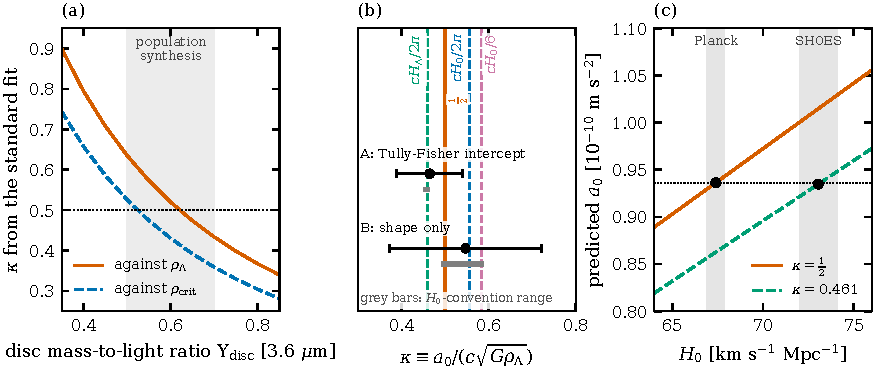
\includegraphics[width=\textwidth]{fig2_kappa.pdf}
\caption{(a) The coefficient returned by the standard fit as a function of the disc mass-to-light ratio, measured against $\rho_\Lambda$ (solid) and against $\rho_{\rm crit}$ (dashed); the band is the range of stellar population models. (b) Estimators A and B (points with $1\sigma$ total errors; grey bars: the range over the $H_0$ adopted for Hubble-flow distances) against the candidate coefficients of Table~\ref{tab:cands}. (c) The $H_0$ lock: the $a_0$ predicted by $\kappa=1/2$ (solid) and by $\kappa=0.461$ (dashed) as a function of $H_0$ at fixed $\Omega_\Lambda$. The two black points, at the Planck and SH0ES values of $H_0$, coincide to 0.2 per cent.}
\label{fig:kappa}
\end{figure*}

\begin{figure*}
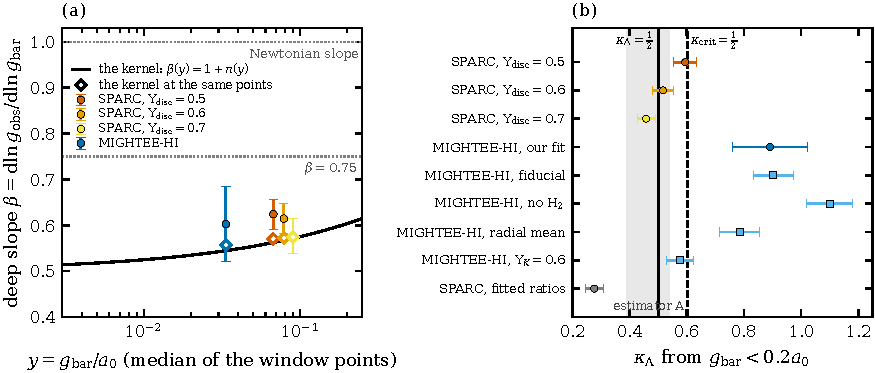
\includegraphics[width=\textwidth]{fig_deep.pdf}
\caption{The deep regime in two surveys. (a) The slope of the relation. The curve is equation~(\ref{eq:beta}). Filled points are the median per-galaxy slopes of SPARC, at three disc mass-to-light ratios, and of MIGHTEE-HI in the window $g_{\rm bar}<0.2a_0$, placed at the median $y$ of their points (the SPARC points are offset by $\pm10$ per cent for clarity), with bootstrap errors. Open diamonds are the same statistic computed from equation~(\ref{eq:nu}) at the same points. The dotted lines mark a slope of 0.75 and the Newtonian slope. (b) The coefficient in the deep regime: SPARC at three disc ratios and our fit to the digitised MIGHTEE-HI points, both in the window (circles); the survey's own fits to all radii under four mass-to-light conventions (squares); and SPARC in the window with mass-to-light ratios fitted to the rotation curves themselves (grey). The solid and dashed lines are $\kappa=1/2$ against $\rho_\Lambda$ and against $\rho_{\rm crit}$; the grey band is estimator A.}
\label{fig:deep}
\end{figure*}

%=====================================================================================================================
\section{The coefficient is degenerate with the Hubble constant}
\label{sec:h0}
Substituting equation~(\ref{eq:rhocrit}) into equations~(\ref{eq:rholambda}) and (\ref{eq:relation}),
\begin{equation}
a_0=\kappa\,c\sqrt{G\,\Omega_\Lambda\frac{3H_0^2}{8\pi G}}=\kappa\,cH_0\sqrt{\frac{3\Omega_\Lambda}{8\pi}} .
\label{eq:lock}
\end{equation}
At fixed $\Omega_\Lambda$ the predicted acceleration depends only on the product $\kappa H_0$. Take the two values of the Hubble constant currently in tension, $67.4$ \citep{Planck2020} and $73.04$ km s$^{-1}$ Mpc$^{-1}$ \citep{Riess2022}. Their ratio is $0.923$, and the ratio of the two leading coefficients is $0.461/0.500=0.921$. Therefore
\begin{equation}
\frac{a_0(\kappa=0.461,\ H_0=73.04)}{a_0(\kappa=0.500,\ H_0=67.4)}=\frac{0.921}{0.923}=0.998 ,
\end{equation}
and the two combinations predict the same $a_0$ to 0.2 per cent (Fig.~\ref{fig:kappa}c). If the physical matter density $\Omega_mh^2$ is held at its CMB value in place of $\Omega_\Lambda$, the matching coefficient is 0.446, which is 3 per cent from 0.461.

The first statement, that only the product $\kappa H_0$ enters, is exact. The second, that the two candidate coefficients map onto the two measured values of $H_0$, is a numerical coincidence to which we attach no physical meaning. Two things follow. A claim that the coefficient is `exactly one half' is also a claim about $H_0$ and about the distance scale of the galaxies, and should say so. And the coefficient cannot be settled ahead of the Hubble tension: read in reverse at $\kappa=1/2$, estimator A gives $H_0=63\pm10$ km s$^{-1}$ Mpc$^{-1}$ and estimator B $74\pm24$, far too coarse to bear on the tension. We record the degeneracy because any future derivation of $\kappa$ will have to confront it.

%=====================================================================================================================
\section{The redshift test}
\label{sec:ztest}
The value of $\kappa$ cannot distinguish $\rho_\Lambda$ from $\rho_{\rm crit}$, nor either from an emergent scale. The redshift dependence can. We define
\begin{equation}
\Delta(z)\equiv\log_{10}\frac{a_0(z)}{a_0(0)} .
\end{equation}

\subsection{Three laws}
\label{sec:laws}
\emph{(a) A scale anchored to $\Lambda$.} The cosmological constant does not evolve, so $\rho_\Lambda$ and $a_0$ are the same at every redshift:
\begin{equation}
\Delta_\Lambda(z)=0 .
\label{eq:lawflat}
\end{equation}
This is the content of the hypothesis, not evidence for it. Plain MOND, in which $a_0$ is simply a constant of nature, makes the same prediction. What the $\Lambda$ anchor adds is a reason for the constancy, and with it the exclusion of law (b).

\emph{(b) A scale anchored to the critical density.} Replacing $\rho_\Lambda$ by $\rho_{\rm crit}(z)=3H^2(z)/8\pi G$ gives $a_0\propto H(z)$. With $E(z)\equiv H(z)/H_0=[\Omega_m(1+z)^3+\Omega_\Lambda]^{1/2}$,
\begin{equation}
\Delta_H(z)=\log_{10}E(z) .
\label{eq:lawH}
\end{equation}
At $z=2.5$, $E^2=0.315\times3.5^3+0.685=14.19$, so $E=3.77$ and $\Delta_H=+0.58$.

\emph{(c) The emergent scale of $\Lambda$CDM haloes.} In $\Lambda$CDM the characteristic acceleration of the relation is inherited from dark-matter haloes. Appendix~\ref{app:nfw} shows that the central acceleration of an NFW halo \citep{NFW1997} of mass $M_{200}$ and concentration $c_{200}$ is
\begin{equation}
g_{\max}=\frac{100^{2/3}}{2}\,(GM_{200})^{1/3}H^{4/3}(z)\,\frac{c_{200}^2}{f(c_{200})},
\label{eq:gmax}
\end{equation}
where $f(x)=\ln(1+x)-x/(1+x)$. For $M_{200}=10^{12}\,{\rm M_\odot}$ today this is $8.1\times10^{-11}$ m s$^{-2}$, close to $a_0$, which is part of the reason that galaxies in $\Lambda$CDM haloes show an $a_0$-like scale \citep{Navarro2017}. At fixed halo mass,
\begin{equation}
\Delta_{\rm halo}(z)=\tfrac43\log_{10}E(z)+\log_{10}\frac{[c^2/f(c)]_z}{[c^2/f(c)]_0} .
\label{eq:lawhalo}
\end{equation}
The first term rises, because haloes of a given mass were denser in the past. The second falls, because they were less concentrated. With the concentration--mass relation of \citet{DuttonMaccio2014}, $c_{200}$ falls from 8.4 to 3.9 between $z=0$ and $2.5$ and
\begin{equation}
\Delta_{\rm halo}(2.5)=0.768-0.440=+0.33 ,
\end{equation}
a factor 2.13. This one number should not be over-read, and Table~\ref{tab:laws} shows why. The value runs from $+0.23$ to $+0.46$ over $M_{200}=10^{11}$--$10^{13}\,{\rm M_\odot}$ and the relations of \citet{DuttonMaccio2014} and \citet{Duffy2008}. A different structural scaling, the Tully--Fisher ratio $V_{\max}^4/GM$ at a fixed ratio of baryonic to halo mass, gives $+0.56$ (Appendix~\ref{app:nfw}). Hydrodynamical simulations point the same way: \citet{KellerWadsley2017} find that the simulated relation is not constant with redshift, and in the Magneticum simulations the best-fitting $a_0$ rises by a factor of about three between $z=0$ and $2.3$ \citep{Mayer2023}, which is $+0.48$ dex. Every $\Lambda$CDM estimate is a rise of $0.2$--$0.6$ dex at $z=2.5$. We adopt $+0.33$ as the decision value because it is near the low end, and a smaller rise is harder to tell from none.

\emph{(d) If dark energy evolves.} Law (a) assumes a true cosmological constant. If instead $a_0$ followed an evolving dark-energy density, $a_0\propto\sqrt{\rho_{\rm DE}(z)}$, then for the $w_0w_a$ fits of \citet{DESI2025}
\begin{equation}
\frac{\rho_{\rm DE}(z)}{\rho_{\rm DE}(0)}=(1+z)^{3(1+w_0+w_a)}\exp\!\Big[-\frac{3w_az}{1+z}\Big]
\end{equation}
gives $\Delta=-0.09$ to $-0.11$ at $z=2.5$ for the three supernova combinations. This is not our prediction. We quote it to show that the test is robust to the question: the alternatives to constancy differ from it by $+0.3$ to $+0.6$ dex, while this differs by $-0.1$.

\begin{table}
\caption{$\Delta(z)=\log_{10}[a_0(z)/a_0(0)]$ in dex for the laws of Section~\ref{sec:laws}. The halo law is for $M_{200}=10^{12}\,{\rm M_\odot}$ with the concentrations of \citet{DuttonMaccio2014}; the bracket is the range over $10^{11}$--$10^{13}\,{\rm M_\odot}$ and the relations of \citet{DuttonMaccio2014} and \citet{Duffy2008}. The last column is the density mapping of Section~\ref{sec:laws}(d) for the DESI+CMB+DESY5 fit.}
\label{tab:laws}
\begin{tabular}{cccccc}
\toprule
$z$ & $\Lambda$ & $H(z)$ & halo & halo, range & $\sqrt{\rho_{\rm DE}}$\\
\midrule
1.0 & 0 & $+0.25$ & $+0.09$ & $[+0.05,+0.16]$ & $+0.00$\\
2.0 & 0 & $+0.48$ & $+0.25$ & $[+0.16,+0.37]$ & $-0.07$\\
2.5 & 0 & $+0.58$ & $+0.33$ & $[+0.23,+0.46]$ & $-0.10$\\
3.0 & 0 & $+0.66$ & $+0.41$ & $[+0.29,+0.54]$ & $-0.13$\\
\bottomrule
\end{tabular}
\end{table}

\begin{figure}
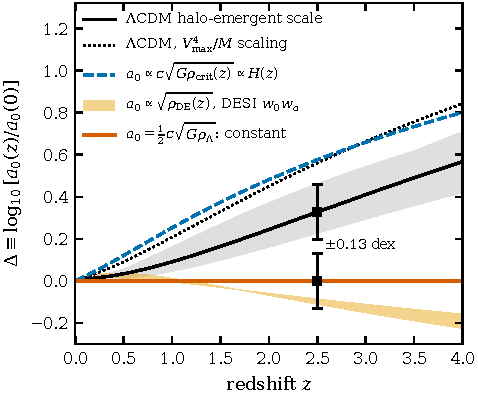
\includegraphics[width=\columnwidth]{fig3_laws.pdf}
\caption{$\Delta(z)$ for the laws of Section~\ref{sec:laws}: a scale anchored to $\Lambda$ (thick horizontal line), a scale anchored to the critical density (dashed), and the $\Lambda$CDM halo-emergent scale (solid black; grey band: range over halo mass and concentration--mass relation; dotted: the $V_{\max}^4/M$ scaling). The narrow shaded band is the density mapping under the DESI DR2 $w_0w_a$ fits, shown for scale. The two squares at $z=2.5$ mark the decision values $0$ and $+0.33$ with error bars of $\pm0.13$ dex.}
\label{fig:laws}
\end{figure}

\subsection{The statistic, and why the depth of the galaxy matters}
\label{sec:amp}
Given $g_{\rm obs}$ and $g_{\rm bar}$ at one radius of one galaxy, equation~(\ref{eq:nu}) can be solved for $a_0$ exactly: find the $y$ for which $\nu(y)=g_{\rm obs}/g_{\rm bar}$ and set
\begin{equation}
\hat a_0=\frac{g_{\rm bar}}{y} .
\label{eq:invert}
\end{equation}
Unlike the deep-regime formula $g_{\rm obs}^2/g_{\rm bar}$, this is unbiased at any acceleration. Its precision is another matter. Take the logarithm of $\nu(y)=g_{\rm obs}/g_{\rm bar}$ and differentiate, writing $n\equiv d\ln\nu/d\ln y$:
\begin{equation}
n\,d\ln y=d\ln g_{\rm obs}-d\ln g_{\rm bar} .
\end{equation}
Since $d\ln\hat a_0=d\ln g_{\rm bar}-d\ln y$,
\begin{equation}
d\ln\hat a_0=-\frac1n\,d\ln g_{\rm obs}+\Big(1+\frac1n\Big)d\ln g_{\rm bar},\qquad n=-\frac{\sqrt y/2}{e^{\sqrt y}-1} .
\label{eq:amp}
\end{equation}
Errors in the kinematics are therefore multiplied by $A_{\rm obs}=1/|n|$, and errors in the baryonic mass by $A_{\rm bar}=A_{\rm obs}-1$. In the deep regime $n\to-1/2$, so $A_{\rm obs}=2$ and $A_{\rm bar}=1$: the familiar $\hat a_0=g_{\rm obs}^2/g_{\rm bar}$, in which a velocity error enters four times. Towards high acceleration $n\to0$ and both factors diverge, because there the relation is $g_{\rm obs}=g_{\rm bar}$ and no longer contains $a_0$ (Table~\ref{tab:amp}, Fig.~\ref{fig:amp}).

\begin{table}
\caption{Error amplification of equation~(\ref{eq:invert}). The last column is the error on $\log_{10}\hat a_0$ for a 5 per cent velocity error and a 0.10 dex baryonic-mass error.}
\label{tab:amp}
\begin{tabular}{ccccc}
\toprule
$y=g_{\rm bar}/a_0$ & $n$ & $A_{\rm obs}$ & $A_{\rm bar}$ & $\sigma(\log_{10}\hat a_0)$\\
\midrule
0.01 & $-0.475$ & 2.1 & 1.1 & 0.14\\
0.1 & $-0.425$ & 2.4 & 1.4 & 0.17\\
0.3 & $-0.376$ & 2.7 & 1.7 & 0.20\\
1.0 & $-0.291$ & 3.4 & 2.4 & 0.29\\
3.0 & $-0.186$ & 5.4 & 4.4 & 0.50\\
6.4 & $-0.110$ & 9.1 & 8.1 & 0.90\\
\bottomrule
\end{tabular}
\end{table}

This is why existing samples cannot decide between the laws. The star-forming galaxies with resolved kinematics at $z\sim1$--$2.5$ are massive and compact. In the largest homogeneous sample, RC100 \citep{NestorShachar2023}, the median is $y=1.45$, the central 68 per cent lie in $0.33<y<5.3$, and only 15 of 99 galaxies lie below $y=0.3$. At the median, a baryonic-mass uncertainty of 0.2 dex, typical at these redshifts, becomes 0.6 dex in $a_0$, which is larger than any of the separations in Table~\ref{tab:laws}. Tully--Fisher zero points at high acceleration suffer from the same dilution, and in addition are degenerate with the evolution of disc sizes. The baryonic zero-point offsets of $-0.44$ and $-0.27$ dex at $z\simeq0.9$ and $2.3$ found by \citet{Ubler2017} therefore cannot be read as changes of $a_0$.

\begin{figure}
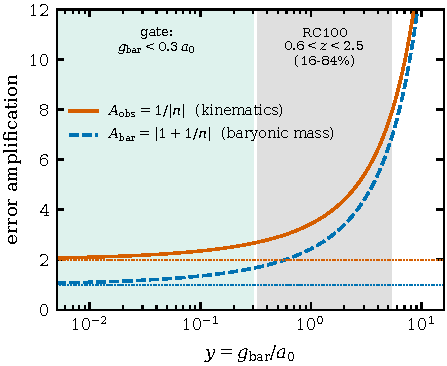
\includegraphics[width=\columnwidth]{fig4_amplification.pdf}
\caption{The factors by which errors in the kinematics ($A_{\rm obs}$, solid) and in the baryonic mass ($A_{\rm bar}$, dashed) are amplified when $a_0$ is inferred through equation~(\ref{eq:invert}). Dotted lines mark the deep limits, 2 and 1. The grey band is the central 68 per cent of the RC100 sample; the shaded region on the left is the gate proposed in Section~\ref{sec:design}.}
\label{fig:amp}
\end{figure}

\subsection{What existing data say}
\label{sec:existing}
\emph{A closed-form inversion of RC100.} \citet{NestorShachar2023} tabulate, for 100 galaxies at $0.6<z<2.5$, the circular velocity at the effective radius and the dark-matter fraction inside it, $f_{\rm DM}\equiv V_{\rm DM}^2/V_c^2$. For this quantity equation~(\ref{eq:invert}) has a closed form. By definition $g_{\rm bar}/g_{\rm obs}=1-f_{\rm DM}$, and by equation~(\ref{eq:nu}) the same ratio is $1/\nu=1-e^{-\sqrt y}$. Therefore
\begin{equation}
e^{-\sqrt y}=f_{\rm DM}\ \Longrightarrow\ y=\Big[\ln\frac1{f_{\rm DM}}\Big]^2\ \Longrightarrow\ \hat a_0=\frac{(1-f_{\rm DM})\,g_{\rm obs}}{[\ln(1/f_{\rm DM})]^2} .
\label{eq:rc100}
\end{equation}
No mass model enters beyond the published $f_{\rm DM}$. The inversion is defined for 99 galaxies (Fig.~\ref{fig:rc100}). The median is $\hat a_0=1.4\times10^{-10}$ m s$^{-2}$ with a scatter of 0.4 dex, as large as Table~\ref{tab:amp} leads one to expect. A straight-line fit gives
\begin{equation}
\frac{d\log_{10}\hat a_0}{dz}=-0.11\pm0.06 .
\end{equation}
The mean slopes of laws (b) and (c) over this range are $+0.23$ and $+0.13$. The inversion itself does not manufacture a flat trend: dark fractions generated from equation~(\ref{eq:nu}) on the real redshifts and accelerations, with injected slopes of 0, $+0.13$ and $+0.23$ and 0.05 of noise in $f_{\rm DM}$, return those slopes to 0.01.

Nevertheless the result is not a measurement, for four reasons. First, it restates the published decline of $f_{\rm DM}$ with redshift and inherits the inputs of the original fits: stellar mass-to-light ratios, gas masses from scaling relations and halo priors. Secondly, the sample is selected differently at different redshifts. Controlling for the measured $g_{\rm obs}$ gives $-0.14\pm0.06$; controlling for the inferred $y$ gives $+0.01\pm0.05$, a control that also absorbs part of any real signal, since a change of $a_0$ changes $y$. Across these treatments the halo law is disfavoured at $2.6\sigma$ to $4.3\sigma$ and the $H(z)$ law at $4.7\sigma$ or more.

Thirdly, and decisively, the verdict depends on the redshift calibration of the baryonic masses, which enters every $f_{\rm DM}$. Suppose the baryonic masses carry a drift of $\beta$ dex per unit redshift about the mean redshift, so that each $g_{\rm bar}$ is multiplied by $10^{\beta(z-\bar z)}$. For $\beta=-0.05$, a factor of 1.1 at either end of the range, the fitted slope moves from $-0.11$ to $+0.02$ and the halo law comes within $2\sigma$. For $\beta=-0.10$ the slope is $+0.16\pm0.07$, which puts constancy $2.3\sigma$ off. One galaxy that sits exactly at the edge of the inversion, $f_{\rm DM}=0.02$, moves the slope by $0.4\sigma$ on its own. Fourthly, the pattern is not reproduced by an independent sample. For 117 galaxies of KMOS$^{\rm 3D}$ with circular velocities from \citet{Ubler2017}, sizes from the survey catalogue \citep{Wisnioski2019} and gas masses from scaling relations (93 of them not in RC100), every model leaves residuals that fall with redshift, the constant-$a_0$ model included. The reason is common to all models: at $z>1.9$ between 27 and 54 per cent of these galaxies rotate more slowly than their own Newtonian baryons would require, which no model that adds gravity to the baryons can fit. The existing rotation curves at $z\sim1$--$2.5$ therefore decide nothing between the laws of Table~\ref{tab:laws}. Their limiting input is the baryonic mass, and a decisive sample needs gas masses measured galaxy by galaxy.

\emph{The MUSE lensed sample at $z\simeq1$.} Two analyses of one survey point in opposite directions. \citet{Jeanneau2026} find that the baryonic Tully--Fisher zero point of 95 lensed galaxies at $z\simeq1$ has changed by $0.00\pm0.06$ dex with respect to $z=0$; many of these galaxies are in the low-acceleration regime, so at face value this favours constancy. \citet{Ciocan2026} fit the radial acceleration relation of 79 galaxies at $0.33<z<1.44$ and find $a_0(z\simeq1)=(2.38\pm0.10)\times10^{-10}$ m s$^{-2}$, which is $\Delta\simeq+0.3$ relative to the local $1.2\times10^{-10}$ m s$^{-2}$. Taken at face value that is a rise as large as the $H(z)$ law ($+0.25$ at $z=1$), and it disfavours constancy: it is the strongest existing evidence against a $\Lambda$-anchored scale. In the catalogue of \citet{Jeanneau2026} the atomic and molecular gas masses come from scaling relations and make up a median 70 per cent of $M_b$, a coherent uncertainty of order 0.2 dex, comparable to the difference between the two analyses. We regard $z\simeq1$ as undecided, and we note that there the halo-emergent law ($+0.09$) cannot be told from constancy by either analysis; the laws separate at higher redshift (Fig.~\ref{fig:laws}).

\emph{Rotation curves at $z\sim2$.} \citet{Milgrom2017} showed that the outer rotation curves of the massive discs of \citet{Genzel2017} are compatible with the local $a_0$ and disfavour a value several times larger. It is subject to the same limits as the RC100 check: high accelerations and model-dependent baryonic masses.

\begin{figure}
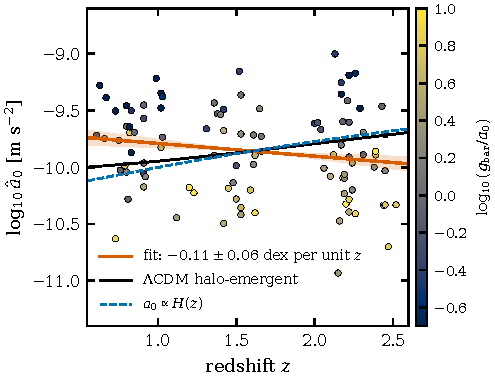
\includegraphics[width=\columnwidth]{fig5_rc100.pdf}
\caption{The acceleration scale inferred from the RC100 dark-matter fractions through equation~(\ref{eq:rc100}), for 99 galaxies, coloured by the acceleration at which each is measured. The band is the fitted trend with its $1\sigma$ slope error. The thin solid and dashed lines are the halo-emergent and $H(z)$ laws, normalised at the mean redshift. The anticorrelation of $\hat a_0$ with $y$ is the signature of noise in $f_{\rm DM}$, which moves the two in opposite directions. The trend is conditional on the redshift calibration of the baryonic masses (Section~\ref{sec:existing}): a drift of $-0.05$ dex per unit redshift brings the halo law within $2\sigma$.}
\label{fig:rc100}
\end{figure}

\subsection{The measurement that decides}
\label{sec:design}
\emph{The gate.} Table~\ref{tab:amp} shows that a galaxy is useful only if it is measured at low acceleration. We propose $g_{\rm bar}(R_{\rm out})<0.3a_0$, where $A_{\rm obs}\le2.7$ and $A_{\rm bar}\le1.7$. With $g_{\rm bar}=\Gamma GM_b/R^2$ and $\Gamma\simeq1.2$ this reads
\begin{equation}
M_b<1.8\times10^{8}\,{\rm M_\odot}\,\Big(\frac{R_{\rm out}}{\rm kpc}\Big)^2 ,
\end{equation}
for example $M_b=5\times10^{9}\,{\rm M_\odot}$ traced to 6 kpc. Such galaxies rotate at $V_f\simeq85$--$130$ km s$^{-1}$. At $z\simeq2.5$ they can be resolved only with the help of gravitational lensing, which adds a requirement on the lens model: a magnification uncertainty below about 0.05 dex (see the budget below). Rotation must dominate ($V/\sigma>1.5$ from a forward-modelled fit), the inclination should be between $35^\circ$ and $75^\circ$, and the gas mass must be measured and not inferred from a scaling relation. A practical sequence is a JWST NIRSpec integral-field observation first, to establish rotation and bound the acceleration (H$\alpha$ and [O\,{\sc iii}] fall together in the G235H grating for $2.3<z<3.8$), followed by ALMA CO(3--2), which falls in Band 3 for $2.0<z<3.1$ and gives the molecular gas mass and a second kinematic tracer. We know of no published object that passes every gate. In a ledger of candidates re-derived from the primary papers, the only object at $z\geq2$ that could pass the acceleration gate is OLAS M0717-02064 \citep{Hirtenstein2019}: $z=2.07$, magnification 6.5, $\log_{10}M_*/{\rm M_\odot}=8.1$, and rotation-supported with $v/\sigma=1.6$. It lies just below the preferred redshift window, where Table~\ref{tab:laws} still separates the laws by 0.25 dex, and it has not been observed with JWST. Its gas mass and the uncertainty of its lens model are not yet measured. The gas mass is the input to watch: the KMOS$^{\rm 3D}$ comparison of Section~\ref{sec:existing} shows that scaling-relation gas masses can carry a redshift-dependent error large enough to decide the test on their own.

\emph{How many galaxies?} For two exactly specified predictions a distance $\Delta$ apart and a Gaussian error $\sigma$, the expected logarithm of the likelihood ratio when one of them is true is $\Delta^2/2\sigma^2$. Odds of 20:1 \citep[strong evidence on the scale of][]{KassRaftery1995} therefore require
\begin{equation}
\sigma\le\frac{\Delta}{\sqrt{2\ln20}}=\frac{\Delta}{2.45} ,
\label{eq:sigma}
\end{equation}
that is, $0.13$ dex for $\Delta=0.33$ and $0.24$ dex for $\Delta=0.58$. For a single galaxy this is too optimistic, because two sources of scatter must be added to the measurement error $\sigma_{\rm m}$. The relation has an intrinsic scatter of about 0.034 dex in $g_{\rm obs}$ \citep{Desmond2023}, which equation~(\ref{eq:amp}) amplifies to $\sigma_{\rm int}=0.08$--$0.09$ dex in $\hat a_0$ for $y=0.1$--$0.3$. And under the $\Lambda$CDM hypothesis haloes of a given mass scatter by 0.11 dex in concentration \citep{DuttonMaccio2014}, which through equation~(\ref{eq:lawhalo}) is $\sigma_{\rm h}=0.13$ dex in the expectation for one object. With variances $s_0^2=\sigma_{\rm m}^2+\sigma_{\rm int}^2$ under constancy and $s_1^2=s_0^2+\sigma_{\rm h}^2$ under the halo law, the expected log-odds from $N$ galaxies when constancy is true are
\begin{equation}
\langle\ln B\rangle=N\Big[\ln\frac{s_1}{s_0}-\frac12+\frac{s_0^2+\Delta^2}{2s_1^2}\Big],
\label{eq:lnB}
\end{equation}
and the expression with $s_0\leftrightarrow s_1$ applies when the halo law is true. Table~\ref{tab:odds} gives the smaller of the two. One galaxy at 0.13 dex yields only 4:1. Two galaxies at 0.10 dex, three at 0.13 dex or four at 0.20 dex exceed 20:1. Against the $H(z)$ law the requirement is looser by a factor of three in variance. An earlier deposited design of this test \citep{Zimmerman2026a0z} quoted a single object at 0.13 dex; the present requirement, which includes both scatters, supersedes it.

\begin{table}
\caption{Expected odds between a constant $a_0$ and the halo-emergent rise of $+0.33$ dex at $z=2.5$, for $N$ galaxies passing the gate, each with measurement error $\sigma_{\rm m}$ on $\log_{10}\hat a_0$, including intrinsic scatter (0.09 dex) and halo-to-halo scatter (0.13 dex). Entries are the smaller of the two cases (constancy true; halo law true).}
\label{tab:odds}
\begin{tabular}{ccccc}
\toprule
$\sigma_{\rm m}$ [dex] & $N=1$ & $N=2$ & $N=3$ & $N=4$\\
\midrule
0.08 & 6:1 & 37:1 & 220:1 & 1300:1\\
0.10 & 5:1 & 25:1 & 120:1 & 610:1\\
0.13 & 4:1 & 14:1 & 53:1 & 200:1\\
0.20 & 2:1 & 5:1 & 13:1 & 29:1\\
\bottomrule
\end{tabular}
\end{table}

\emph{The error budget.} Gravitational lensing conserves surface brightness, so $g_{\rm bar}\propto M_b/R^2$ does not depend on the magnification $\mu$, while $g_{\rm obs}=V^2/R$ scales as $\mu^{1/2}$ through the radius. Equation~(\ref{eq:amp}) then gives
\begin{equation}
\sigma_{\rm m}^2=A_{\rm obs}^2\Big[\Big(\frac{2}{\ln10}\frac{\delta V}{V}\Big)^2+\Big(\frac12\delta\log_{10}\mu\Big)^2\Big]+A_{\rm bar}^2\big(\delta\log_{10}M_b\big)^2 ,
\end{equation}
where $\delta\log_{10}M_b$ is the error of the mass scale at fixed magnification. At $y=0.2$ ($A_{\rm obs}=2.5$, $A_{\rm bar}=1.5$), three budgets reproduce the rows of Table~\ref{tab:odds}: $\sigma_{\rm m}=0.10$ dex needs $(\delta V/V,\delta\log_{10}M_b,\delta\log_{10}\mu)=(2.5$ per cent$,0.04,0.04)$; $0.13$ dex needs $(3$ per cent$,0.06,0.05)$; and $0.20$ dex needs $(5$ per cent$,0.10,0.06)$. The first two are beyond present practice for the baryonic mass, since the conversion from CO luminosity to molecular mass is rarely known to 0.06 dex. The third is within reach, and four such galaxies give 29:1. The realistic programme is therefore four galaxies at 0.20 dex.

\emph{The decision rule.} The statistic is the mean of $\Delta=\log_{10}[\hat a_0/a_0(0)]$ over the galaxies that pass the gate, with $\hat a_0$ from equation~(\ref{eq:invert}) and $a_0(0)$ fixed beforehand from the local relation using the same mass-to-light conventions. A result near $0$ supports constancy: law (a), and with it plain MOND. A result near $+0.33$ or above supports an emergent or $H(z)$-coupled scale and excludes equation~(\ref{eq:relation}) with a constant $\rho_\Lambda$. A result inconsistent with all of them counts against all of them. No nuisance term may be introduced after the data are seen. Because $a_0(0)$ and $\hat a_0(z)$ are obtained with the same function and conventions, the test does not depend on $\kappa$ or on $H_0$, and it depends on the choice of transition function only weakly provided $a_0(0)$ is calibrated on local galaxies at matching accelerations. It does depend on the stellar and gas mass scales being on a common calibration at both epochs.

%=====================================================================================================================
\section{What the relation does not explain}
\label{sec:limits}
\emph{The coefficient is not derived.} We know of no derivation of $\kappa=1/2$. The simplest physical identification, equating the Unruh temperature of $a_0$ with the temperature of the de Sitter horizon, gives $a_0=cH_\Lambda$, which is six times too large; the form $cH_\Lambda/2\pi$ ($\kappa=0.461$) is allowed by the data as readily as $1/2$ (Table~\ref{tab:cands}). A separate analysis shows that local relativistic actions for MOND of the aether--scalar class cannot fix the coefficient at all, because the additive constant of the MOND Lagrangian is degenerate with $\Lambda$ \citep{Zimmerman2026kappa}. Nothing in this paper changes if $\kappa$ lies anywhere in $0.45$--$0.58$.

\emph{A scale is not a dynamics.} Equation~(\ref{eq:relation}) fixes a number. It does not say whether the low-acceleration behaviour of galaxies is a modification of gravity, a modification of inertia, or a regularity of dark matter. It is therefore silent on gravitational lensing, the cosmic microwave background, the growth of structure, the external field effect \citep{Chae2020} and the Solar System. In particular, equation~(\ref{eq:nu}) is used here only to describe rotation curves; read as a modified-gravity law and extrapolated to Solar System accelerations it is constrained by planetary ephemerides \citep{Hees2016}.

\emph{Clusters of galaxies.} Dynamics governed by $a_0$ leave a residual mass discrepancy of about a factor of two in rich clusters \citep{SandersMcGaugh2002,FamaeyMcGaugh2012}. Anchoring $a_0$ to $\Lambda$ does not change that.

\emph{The mass-to-light ratio.} The value $\kappa=1/2$ with $\rho_\Lambda$ is tenable only if $\Upsilon_{\rm disc}\simeq0.6$ at 3.6 $\mu$m (Table~\ref{tab:upsilon}). An independent determination well outside $0.45$--$0.75$ would exclude it. The $\rho_{\rm crit}$ reading needs $\Upsilon_{\rm disc}\simeq0.5$. The deep regime shows how much is at stake: with the SED ratios of MIGHTEE-HI, a $K_s$-band median of 0.35, the coefficient is $0.90\pm0.07$, and with a fixed $\Upsilon_K=0.6$ it is $0.58\pm0.05$ (Section~\ref{sec:deepregime}). The stellar mass calibration, not the number of galaxies, limits this test.

\emph{Constancy is shared.} A constant $a_0$ at $z=2.5$ would not distinguish equation~(\ref{eq:relation}) from a MOND constant of unknown origin. It would exclude the coupling to $H(z)$, which the coincidence $a_0\sim cH_0$ has suggested since 1983, and it would require $\Lambda$CDM to produce an acceleration scale that stays fixed while the haloes that set it evolve.

\emph{Dark energy may not be a constant.} If the evidence for evolving dark energy \citep{DESI2025} is confirmed, $\rho_\Lambda$ in equation~(\ref{eq:relation}) will need redefinition. The redshift test is insensitive to this at the level of 0.1 dex (Section~\ref{sec:laws}d).

%=====================================================================================================================
\section{Conclusions}
\label{sec:conc}
\begin{enumerate}
\item The only acceleration that can be formed from $c$, $G$ and the density of the cosmological constant is $\kappa c\sqrt{G\rho_\Lambda}$. For $\kappa=1/2$ it is $9.36\times10^{-11}$ m s$^{-2}$; the same expression with the critical density is $1.13\times10^{-10}$ m s$^{-2}$. The forms $c^2\sqrt{\Lambda/32\pi}$, $cH_\Lambda/5.79$ and $M_\Lambda^2/2M_{\rm P}$ are identities and carry no separate evidence.
\item On SPARC, $\kappa=0.465\pm0.076$ from the Tully--Fisher intercept with its finite-depth correction, and $0.55\pm0.17$ from a shape-only estimator that is immune to a common distance error but fragile to the bulge mass-to-light ratio. The value $1/2$ is consistent with both, as are $cH_\Lambda/2\pi$ and $cH_0/2\pi$. Injection tests show that each estimator returns a known $a_0$; none echoes an assumed value. The thermal identifications $cH_\Lambda$ and $2cH_\Lambda$ are excluded.
\item In the deep regime, $g_{\rm bar}<0.2a_0$, the per-galaxy slope of SPARC and MIGHTEE-HI agrees with the slope of equation~(\ref{eq:nu}) at the sampled accelerations, within 0.1--$1.6\sigma$, and excludes a slope of 0.75 at more than $4\sigma$. The amplitude follows the stellar mass-to-light convention: $\kappa_\Lambda=0.90\pm0.07$ with the SED ratios of MIGHTEE-HI and $0.58\pm0.05$ with its fixed $\Upsilon_K=0.6$, which is consistent with SPARC. Mass-to-light ratios fitted to the rotation curves themselves lower the deep-regime value by a factor of 1.7 to 2.2 and must not be used.
\item Because stellar and gas masses sum to the baryonic mass, the two calibrations trade against each other and leave a floor $s_\Upsilon s_g/(s_\Upsilon^2+s_g^2)^{1/2}=9.5$ per cent on $a_0$ that no sample size removes. Separating $1/2$ from $0.461$ needs 2.6 per cent.
\item At fixed $\Omega_\Lambda$ only the product $\kappa H_0$ enters the prediction, so $\kappa$ cannot be quoted without $H_0$. By numerical coincidence, $(\kappa,H_0)=(0.500,67.4)$ and $(0.461,73.04)$ give the same $a_0$ to 0.2 per cent.
\item The $\Lambda$ anchor predicts a constant $a_0$. A critical-density anchor predicts $+0.58$ dex at $z=2.5$, and $\Lambda$CDM haloes predict $+0.33$ dex (range $0.2$--$0.6$). Inferring $a_0$ from one galaxy amplifies kinematic errors by $1/|n|$ and mass errors by $1/|n|-1$, factors of 4 and 3 at the accelerations of existing high-redshift samples. This is why those samples do not decide the matter.
\item A closed-form inversion of the 99 usable RC100 galaxies gives $d\log_{10}a_0/dz$ between $-0.14$ and $+0.01$ depending on the control for selection, but a drift of $-0.05$ dex per unit redshift in the baryonic-mass calibration brings the halo-emergent rise within $2\sigma$, and an independent KMOS$^{\rm 3D}$ sample does not reproduce the pattern. At $z\simeq1$ the two analyses of the MUSE lensed survey disagree: one finds a rise of $+0.3$ dex, the strongest existing evidence against constancy, and the other finds no change. Existing high-redshift rotation curves decide nothing; directly measured gas masses are the lever.
\item Two lensed rotators at $z\simeq2.5$ with $g_{\rm bar}<0.3a_0$ measured to 0.10 dex in $a_0$, three at 0.13 dex or four at 0.20 dex decide between constancy and the halo-emergent rise at 20:1 once intrinsic and halo-to-halo scatter are included. One such galaxy does not.
\end{enumerate}

\section*{Acknowledgements}
Generative artificial-intelligence tools were used in this work. Large language models (Anthropic's Claude, used through the Claude Code tool, and in earlier exploratory stages models from OpenAI) assisted with the derivations, with writing the analysis code and with drafting the text. Every quantitative statement is produced by a script that the author has run, the scripts contain checks that can fail, and the author has reviewed the full content and takes sole responsibility for it. The ordering of the observing sequence in Section~\ref{sec:design} was first suggested in an exchange with an OpenAI model. This work made use of the SPARC database \citep{Lelli2016} and of the tables of \citet{NestorShachar2023}. The author received no funding for this work and declares no conflict of interest.

\section*{Data Availability}
All scripts and outputs are in the public repository \url{https://github.com/carlzimmerman/zimmerman-formula}, in the directory \nolinkurl{qwen_claude_field_theory/papers_2026/mnras_submission_2026_v2} (Appendix~\ref{app:repro}). The SPARC data are available at \url{http://astroweb.cwru.edu/SPARC/}. The RC100 table is from \citet{NestorShachar2023}. The MIGHTEE-HI points were digitised from \citet{Varasteanu2025}, and the digitised values are in the repository. Earlier versions of parts of this work are deposited at Zenodo \citep{Zimmerman2026kappa,Zimmerman2026a0z}.

\bibliographystyle{mnras}
\bibliography{references}

\appendix
\section{The acceleration scale of an NFW halo}
\label{app:nfw}
The NFW density profile is $\rho(r)=\rho_s/[x(1+x)^2]$ with $x=r/r_s$. Integrating, the mass inside $r$ is
\begin{equation}
M(<r)=4\pi\rho_sr_s^3\,f(x),\qquad f(x)=\ln(1+x)-\frac{x}{1+x} .
\end{equation}
The halo is bounded at $r_{200}$, inside which the mean density is $200\rho_{\rm crit}(z)$, and the concentration is $c_{200}=r_{200}/r_s$. Dividing $M(<r)$ by $M_{200}=M(<r_{200})$ removes $\rho_s$:
\begin{align}
M(<r)&=M_{200}\,\frac{f(x)}{f(c_{200})},\\
g(r)&=\frac{GM(<r)}{r^2}=\frac{GM_{200}}{f(c_{200})\,r_s^2}\,\frac{f(x)}{x^2} .
\end{align}
For small $x$, $f(x)=x^2/2-2x^3/3+\ldots$, so $f(x)/x^2\to1/2$. The acceleration is therefore largest at the centre, and with $r_s=r_{200}/c_{200}$
\begin{equation}
g_{\max}=\frac{GM_{200}\,c_{200}^2}{2f(c_{200})\,r_{200}^2} .
\label{eq:gmaxA}
\end{equation}
The radius follows from the definition of $M_{200}$ and from $\rho_{\rm crit}(z)=3H^2/8\pi G$:
\begin{align}
M_{200}&=\frac{4\pi}{3}\,200\,\frac{3H^2}{8\pi G}\,r_{200}^3=\frac{100H^2r_{200}^3}{G},\\
r_{200}&=\Big(\frac{GM_{200}}{100H^2}\Big)^{1/3} .
\end{align}
Hence $GM_{200}/r_{200}^2=100^{2/3}(GM_{200})^{1/3}H^{4/3}$, and substituting in equation~(\ref{eq:gmaxA}) gives equation~(\ref{eq:gmax}). At fixed $M_{200}$ the ratio of $g_{\max}$ at redshift $z$ to its value today is equation~(\ref{eq:lawhalo}).

\emph{Numbers.} For $M_{200}=10^{12}\,{\rm M_\odot}$ the relation of \citet{DuttonMaccio2014}, $\log_{10}c_{200}=a+b\log_{10}(M_{200}/10^{12}h^{-1}{\rm M_\odot})$ with $a=0.520+0.385\,e^{-0.617z^{1.21}}$ and $b=-0.101+0.026z$, gives $c_{200}=8.36$ and $r_{200}=212$ kpc at $z=0$, so $g_{\max}=8.1\times10^{-11}$ m s$^{-2}$. At $z=2.5$ it gives $c_{200}=3.85$, $r_{200}=87$ kpc and $g_{\max}=1.72\times10^{-10}$ m s$^{-2}$. The ratio is $2.13$. Term by term: $E^{4/3}=3.767^{4/3}=5.86$, and $[c^2/f(c)]_{2.5}/[c^2/f(c)]_0=18.9/52.0=0.363$.

\emph{A second scaling.} The virial velocity is $V_{200}=(10GM_{200}H)^{1/3}$, and the maximum circular velocity of an NFW halo is $V_{\max}^2=0.216\,V_{200}^2\,c_{200}/f(c_{200})$. The Tully--Fisher-like ratio $V_{\max}^4/GM_b$ at a fixed ratio $M_b/M_{200}$ therefore scales as $E^{4/3}[c/f(c)]^2$. Between $z=0$ and $2.5$ this is a factor $3.64$, or $+0.56$ dex; it is lower by the logarithm of any increase in $M_b/M_{200}$. Both scalings rise, and we use the smaller in the text.

\section{Reproducibility}
\label{app:repro}
The scripts below produce every number in the paper. Each prints its checks as PASS or FAIL and exits with a non-zero status on any failure; \texttt{reproduce\_all.sh} runs them in sequence. The checks in \texttt{paper\_numbers.py} are labelled by kind, because not every check is evidence. Of its 51 checks, 15 are identities: they verify algebra or arithmetic on stated inputs, such as the equivalence of the forms in Section~\ref{sec:forms}, and can fail only through a coding error. Six evaluate published models at stated inputs. Twenty-four can fail on the data. Six are injection tests (Sections~\ref{sec:injection} and \ref{sec:deepregime}), which feed an estimator synthetic data with a known answer. Only the last two kinds carry evidence. Paths are relative to the repository root, and \texttt{v2/} stands for the directory named in the Data Availability statement.
\begin{itemize}
\item \nolinkurl{v2/paper_numbers.py}: Tables~\ref{tab:inputs}, \ref{tab:upsilon}, \ref{tab:shape}, \ref{tab:deep}, \ref{tab:cands}, \ref{tab:laws}, \ref{tab:amp} and \ref{tab:odds}; estimator B; Sections~\ref{sec:floor}, \ref{sec:deepregime}, \ref{sec:h0}, \ref{sec:existing} and \ref{sec:design}; Appendix~\ref{app:nfw}.
\item \nolinkurl{v2/make_figures.py}: Figs~\ref{fig:rar}--\ref{fig:rc100}, built from the functions of the script above.
\item \nolinkurl{real_research/reviews/mi_btfr_intercept_kappa_door_2026.py}: estimator A and Table~\ref{tab:budget}.
\item \nolinkurl{real_research/reviews/mi_distance_free_gbar_estimator_sparc_2026.py}: the earlier form of estimator B with $\Upsilon_{\rm bul}$ fixed, reproduced as a check.
\item \nolinkurl{real_research/dark_sector_2026/L332_kmos3d_trend_replication.py}: the KMOS$^{\rm 3D}$ comparison of Section~\ref{sec:existing}.
\item \nolinkurl{real_research/reviews/kappa_h0_convention_audit_2026.py}: the $H_0$-convention ranges of Sections~\ref{sec:btfr} and \ref{sec:shape}.
\item \nolinkurl{real_research/reviews/deep_a0eff_audit_2026_09_25/}: the audit that traced the fitted mass-to-light ratios of Section~\ref{sec:deepregime} and re-ran the analyses built on them.
\end{itemize}

\bsp
\label{lastpage}
\end{document}
